\chapter{Modelo matemático}

De acuerdo con \cite[p.~14]{Dombre2007}, el diseño y control de robots requiere diversos modelos matemáticos, tales como:

\begin{itemize}
\item Cinemática directa e inversa, es decir, encontrar la posición del efector final en términos de las coordenadas de las articulaciones y viceversa.
\item Cinemática de la velocidad, encontrar la velocidad del efector final en términos de la velocidad de las articulaciones y viceversa.
\item Modelo dinámico, el cual establece la relación entre los torques o fuerzas que ejercen los actuadores y las posiciones, velocidades y aceleraciones de las articulaciones.
\end{itemize}

\begin{figure}
    \centering
    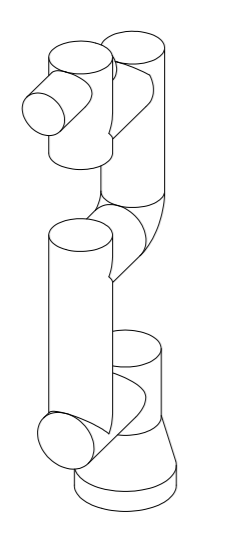
\includegraphics[scale=0.7]{./img/chapter4/robotarmprototype.png}
    \caption{Boceto del brazo robótico propuesto}
    \label{fig:roboticarmprototype}
\end{figure}

En este capítulo se desarrollarán estos modelos matemáticos, los cuales son necesarios para simular y predecir el comportamiento del mismo. 

Para realizar estos modelos, es necesario contar con los parámetros físicos y geométricos del robot, los cuales, para una primera aproximación se mencionarán a continuación.

Como podemos apreciar en el diagrama de requerimientos de la figura \ref{fig:requirementdiagram}, es necesario que el robot tenga seis grados de libertad del tipo revoluta, así, el diagrama de cuerpo libre de la cadena cinemática se expresa en la figura \ref{fig:kinematicchain}.

Otros requerimientos necesarios para el desarrollo del modelo matemático es el alcance total del brazo, el cual deberá ser de mínimo 450 mm, la velocidad, la cuál deberá estar en un rango entre 30 \degree/s y 180 \degree/s, por último, la carga útil deberá ser de 2 kg.

\begin{figure}
    \centering
    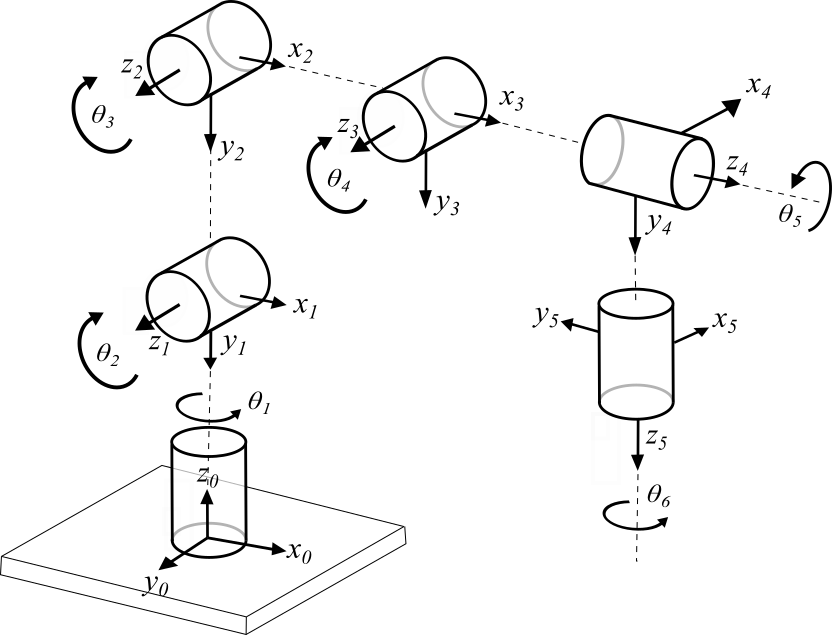
\includegraphics[scale=0.45]{./img/chapter4/kinematicchainv5.png}
    \caption{Cadena cinemática ¿free body diagram?}
    \label{fig:kinematicchain}
\end{figure}

En la figura \ref{fig:roboticarmprototype} podemos ver un boceto del brazo robótico que se planea implementar.

Las distancias, masas e inercia de las articulaciones las podemos observar en la tabla x.

Con estos datos claros, es posible empezar la realización de los modelos matemáticos.

\section{Cinemática directa e inversa}
\subsection{Cinemática directa}

La cinemática directa de un robot se refiere al cálculo de la posición y orientación del marco de referencia del efector final desde sus coordenadas $\theta$. \cite{University2017}

\subsubsection{Matriz de transformación homogénea}

Según \cite{University2017}, existen tres usos principales para una matriz de transformación homogénea:

\begin{enumerate}
  \item Para representar la configuración (posición y orientación) de un cuerpo rígido.
  \item Para cambiar el marco de referencia en el cuál está representado un vector o un \textit{frame}.
  \item Para desplazar un vector o un \textit{frame}.
\end{enumerate}

\begin{figure}
    \centering
    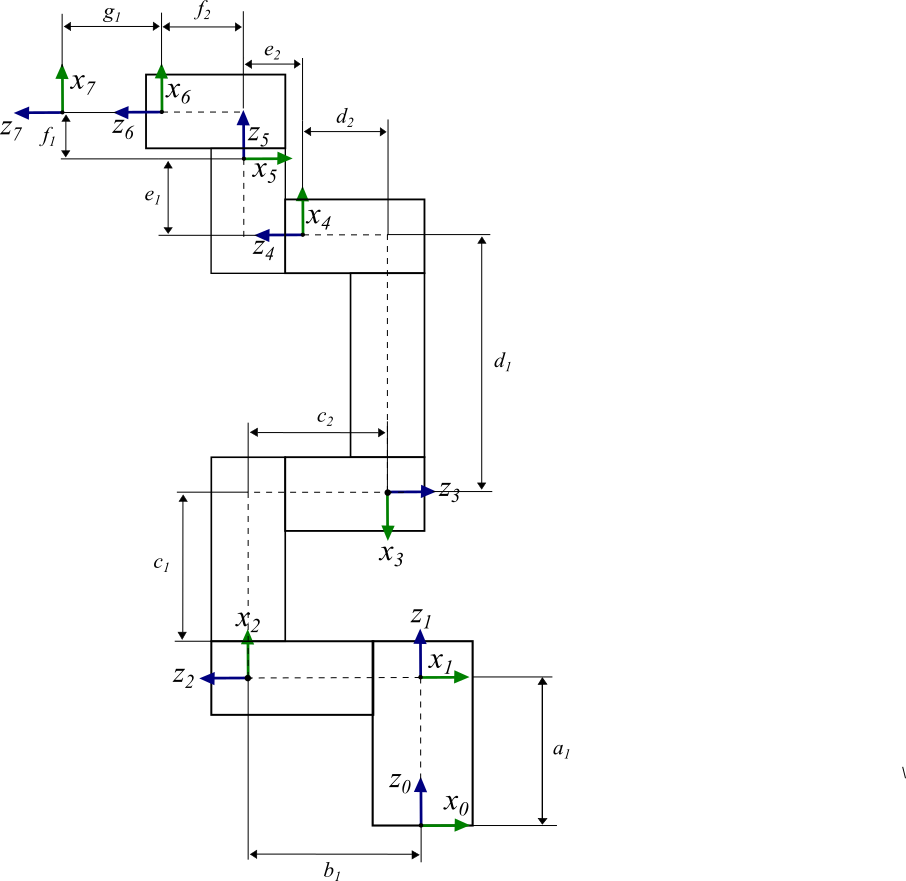
\includegraphics[scale=0.7]{./img/chapter4/kinematicdiagram.png}
    \caption{Diagrama cinemático}
    \label{fig:kinematicchain}
\end{figure}

Para el caso que nos ocupa, necesitamos la matriz de transformación homogénea desde la base fija del robot hasta su efector final, por esto, está descrita con siete marcos de referencia y se obtiene con la ecuación siguiente:

\begin{equation}
\label{eq:forwardkinematicequation}
{}_{0}^{8}T = {}_{0}^{1}T \ {}_{1}^{2}T \ {}_{2}^{3}T \ {}_{3}^{4}T \ {}_{4}^{5}T \ {}_{5}^{6}T {}_{6}^{7}T
\end{equation}

\begin{multicols}{2}
% No hay rotación, sólo traslación
\[
{}_{0}^{1}T = 
\begin{bmatrix}
    1 & 0 & 0 & 0 \\
    0 & 1 & 0 & 0 \\
    0 & 0 & 1 & {a}_1 \\
    0 & 0 & 0 & 1
\end{bmatrix}
\]
% Hay rotación en oreintación y sobre tetha_1 = Rotz*Roty(90)
\[
{}_{1}^{2}T = 
\begin{bmatrix}
    0 & -s_{\theta_1} & c_{\theta_1} & -b_{1}c_{\theta_1}  \\
    0 & c_{\theta_1} & s_{\theta_1} & b_{1}s_{\theta_1} \\
    -1 & 0 & 0 & 0 \\
    0 & 0 & 0 & 1
\end{bmatrix}
\]
% Hay rotación en orientación y sobre tetha_2 = Rotz*Roty(-180)
\[
{}_{2}^{3}T = 
\begin{bmatrix}
    -c_{\theta_2} & -s_{\theta_2} & 0 & c_{1}c_{\theta_2}  \\
    -s_{\theta_2} & c_{\theta_2} & 0 & c_{1}s_{\theta_2} \\
    0 & 0 & -1 & -c_2 \\
    0 & 0 & 0 & 1
\end{bmatrix}
\]
% Hay rotación en orientación y sobre tetha_3 = Rotz*Roty(180)
\[
{}_{3}^{4}T = 
\begin{bmatrix}
    -c_{\theta_3} & -s_{\theta_3} & 0 & -d_{1}c_{\theta_3}  \\
    -s_{\theta_3} & c_{\theta_3} & 0 & d_{1}s_{\theta_3} \\
    0 & 0 & -1 & -d_2 \\
    0 & 0 & 0 & 1
\end{bmatrix}
\]
% Hay rotación en orientación y sobre tetha_4. Rotz*Roty(90)
\[
{}_{4}^{5}T = 
\begin{bmatrix}
    0 & -s_{\theta_4} & c_{\theta_4} & e_{1}c_{\theta_4}  \\
    0 & c_{\theta_2} & s_{\theta_4} & e_{1}s_{\theta_4} \\
    -1 & 0 & 0 & e_2 \\
    0 & 0 & 0 & 1
\end{bmatrix}
\]

\[
{}_{5}^{6}T = 
\begin{bmatrix}
    0 & -s_{\theta_5} & -c_{\theta_5} & -f_{2}c_{\theta_5}  \\
    0 & c_{\theta_5} & -s_{\theta_5} & f_{2}s_{\theta_5} \\
    1 & 0 & 0 & f_1 \\
    0 & 0 & 0 & 1
\end{bmatrix}
\]
% corregir para agregar tetha6
\[
{}_{6}^{7}T = 
\begin{bmatrix}
    1 & 0 & 0 & 0 \\
    0 & 1 & 0 & 0 \\
    0 & 0 & 1 & {g}_1 \\
    0 & 0 & 0 & 1
\end{bmatrix}
\]

\end{multicols}

Para realizar la ecuación \ref{eq:forwardkinematicequation} se programó un algoritmo en MATLAB que tiene como datos de entrada un vector $tetha$ con los seis ángulos de las articulaciones del robot y calcula la posición del efector final. Dicho algoritmo se puede consultar en el Anexo 1.



\subsubsection{Convención de Denavit-Hartenberg}


\begin{table}[h]
\centering
\caption{Parámetros Denavit Hartenberg}
 \label{table:denavithartenberg}
\begin{tabular}{l|l|l|l|l|}
               & $\theta$ [rad] & a [m]    & d [m]   & $\alpha$ [rad]                        \\ 
\hline
Articulación 1 & 0                           & 0        & 0.1519  & $\frac{\pi}{2}$   \\
Articulación 2 & 0                           & -0.24365 & 0       & 0                                                  \\
Articulación 3 & 0                           & -0.21325 & 0       & 0                                                  \\
Articulación 4 & 0                           & 0        & 0.11235 & $\frac{\pi}{2}$   \\
Articulación 5 & 0                           & 0        & 0.08535 & $-\frac{\pi}{2}$  \\
Articulación 6 & 0                           & 0        & 0.0819  & 0                                                 
\end{tabular}
\end{table}

\subsection{Cinemática inversa}
No estoy seguro para que me servirá, si lo hará el software. MoveIt o MATLAB.

\section{Cinemática de la velocidad}


\section{Modelo dinámico}
\subsection{Formulación Lagraniana}
\subsection{Formulación Newton-Euler}